\chapter{Introduction}\label{ch:introduction}

As the global interest in renewable energy increases,
the interest in photo voltaic (PV) arrays grows as well. 
Solar power is a growing source of renewable energy on a global scale \cite{solglob}. \todo[color=c01]{ref}
% http://www.ren21.net/wp-content/uploads/2017/06/170607_GSR_2017_Highlights.pdf
This can be indicated by the growing interest power companies show in building PV parks. 
%\cite{solpowcomp}. \todo[color=c01]{find source}

When generating power with PV arrays,
the initial output is a DC power of varying voltage levels. \todo[color=c01]{find source}
To be able to input the generated power into the stable AC-grid,
without creating disturbances,
the same voltage and frequency as the grid needs to be output. \todo[color=c01]{find source}

\begin{figure}[H]
   \centering
   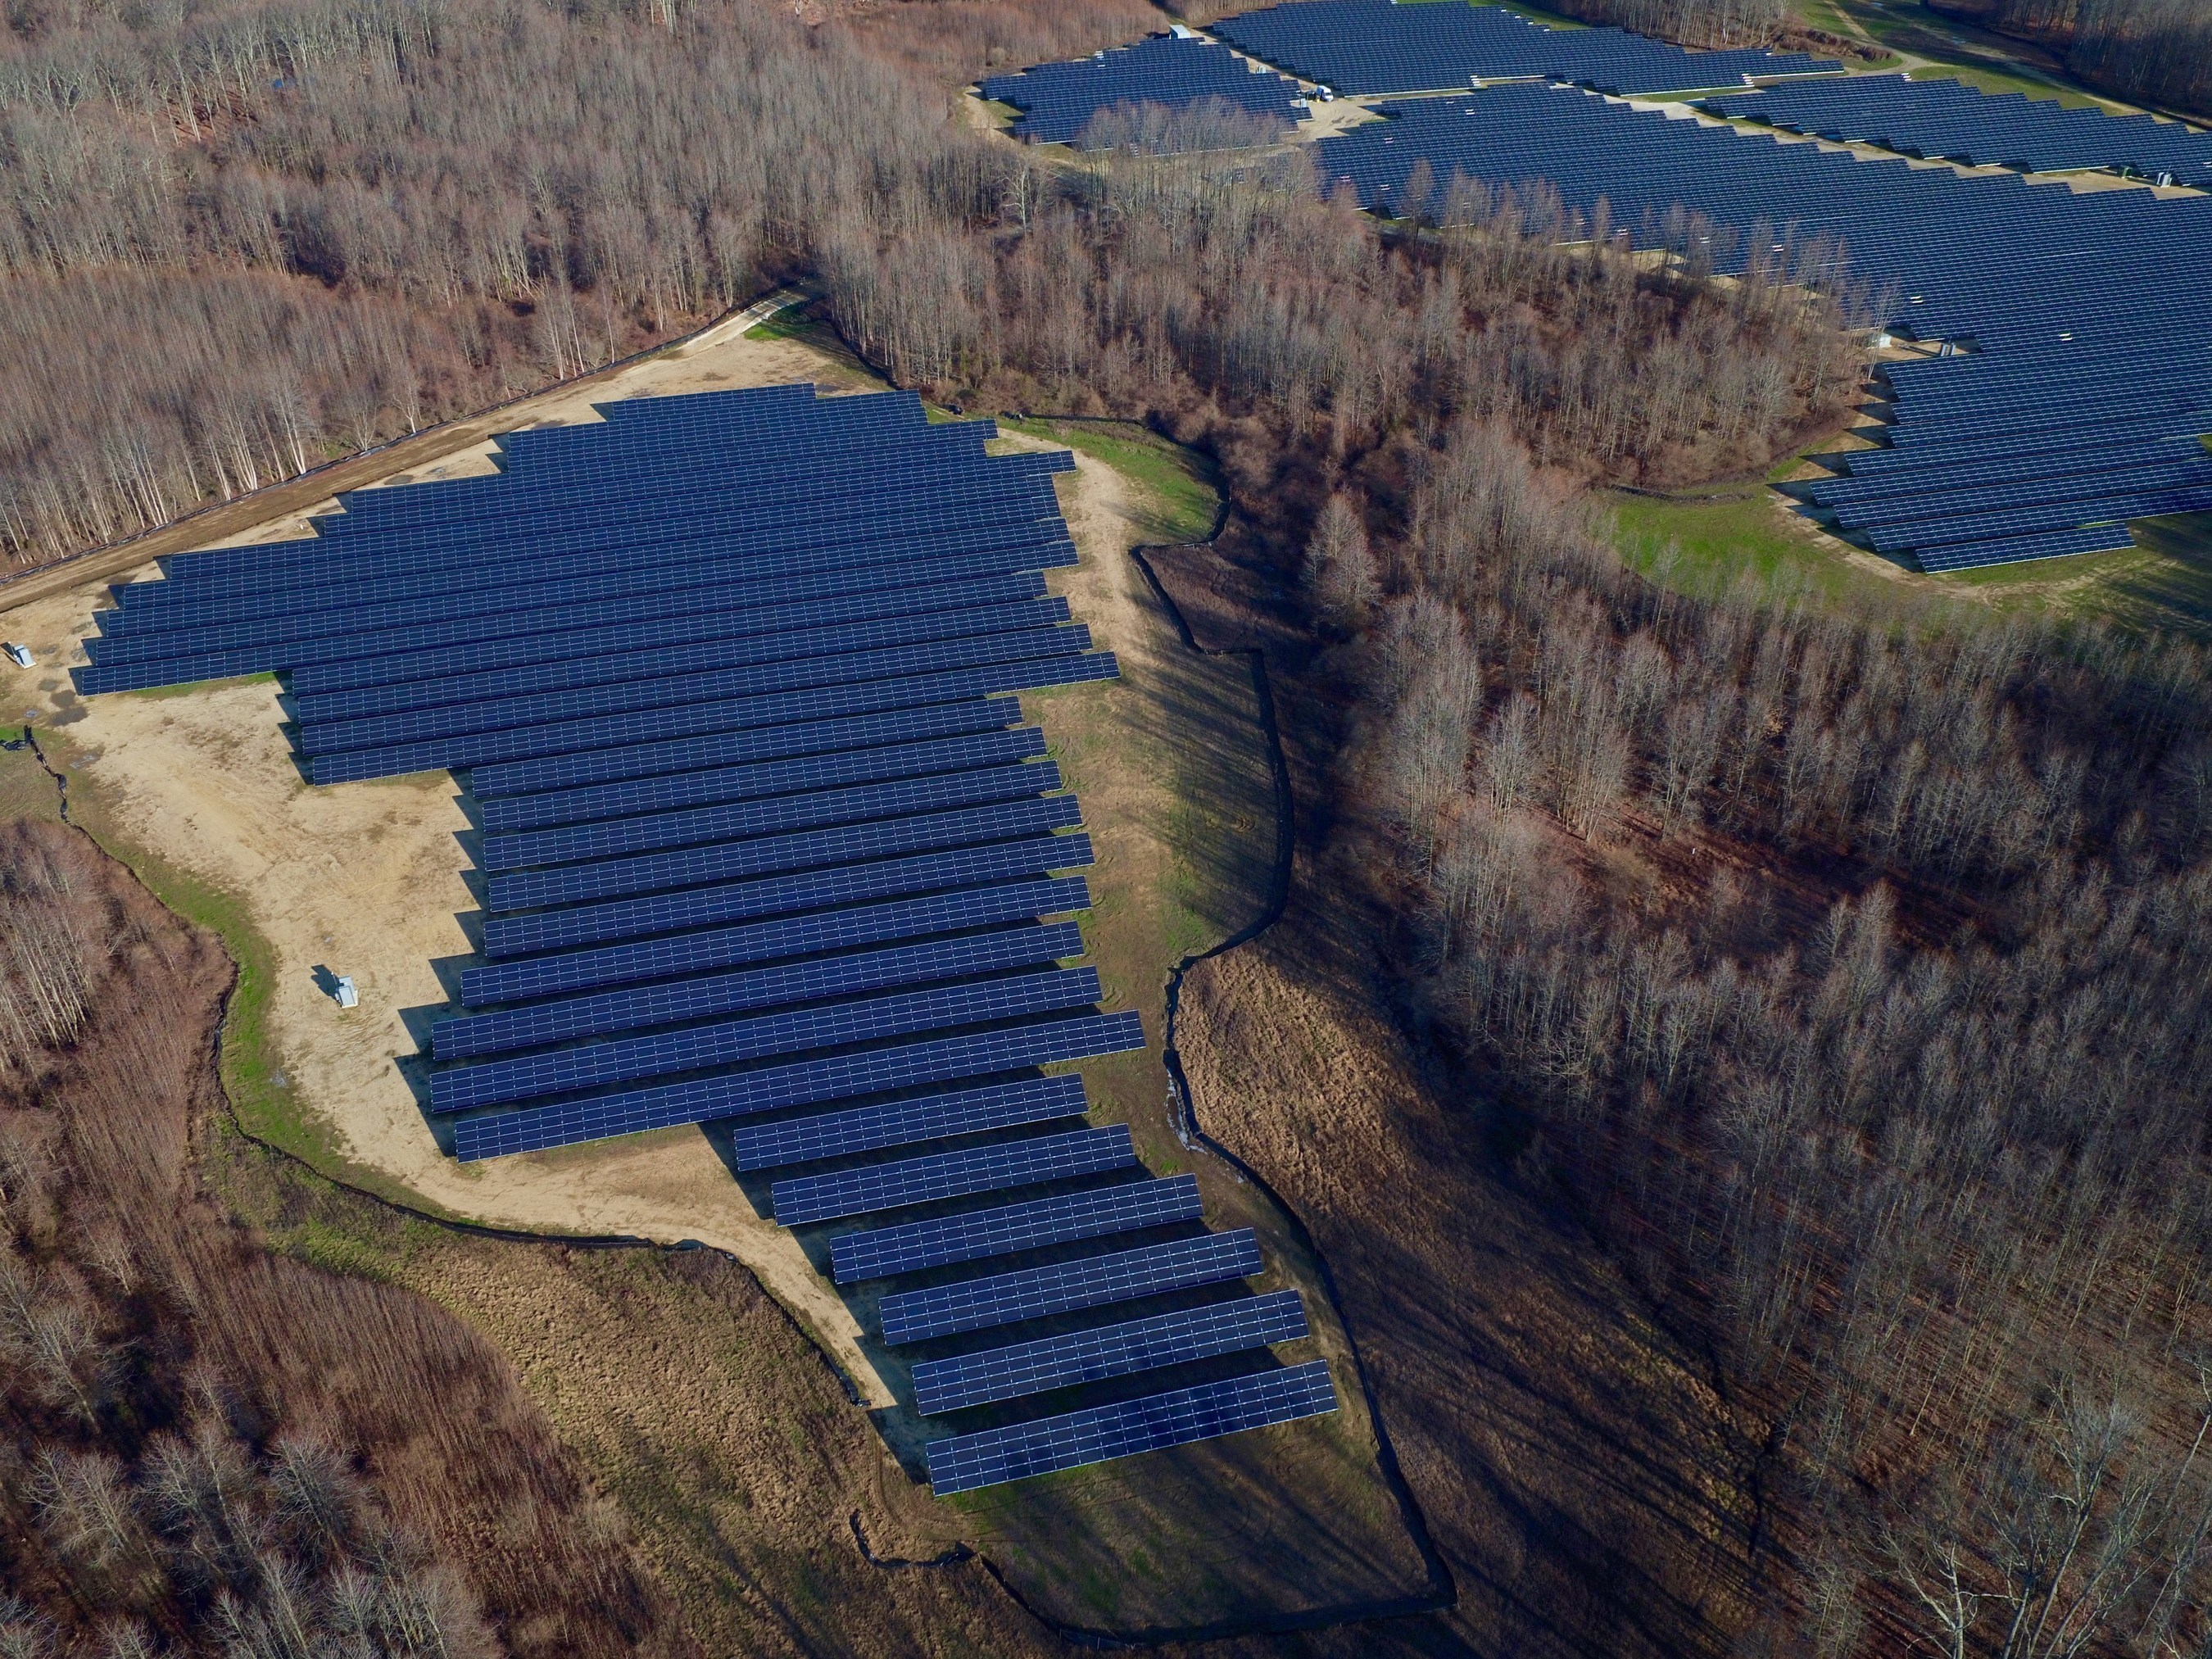
\includegraphics[width=0.8\textwidth]{figures/Problem/solarpark.jpg}
    \caption{12.8 MW Utility Project - the World's Largest Bifacial PV Installation in Eastern US}
	\label{fig:SolarPark}
\end{figure}
\todo[color=c01]{https://www.prnewswire.com/news-releases/sunpreme-deploys-the-worlds-largest-bifacial-pv-installation-for-a-128-mw-utility-project-in-eastern-us-300325989.html}
Commonly this is achieved by two devices,
a DC-DC boost converter (BC) to normalize the voltage
and an DC-AC inverter to generate AC power with the necessary frequency.

In this project we have a look at DC-DC boost converters.
The first part of the project is understanding and simulating common topologies.
The second part is understanding, simulating and building a new topology,
the 2NX Interleaved Boost Converter. \todo[color=c01]{Sanjee's paper is the source}


\section*{Reading Guide}
For readers without an understanding of DC-DC converters,
it is recommended to read the Chapters \ref{ch:basicI}-\ref{ch:basicII}, \todo[color=c01]{ref basic knowledge chapters}
before reading the Chapters \ref{ch:more_advancedI}-\ref{ch:more_advancedII}. \todo[color=c01]{ref advanced chapters}
as these require a deeper understanding.